\section{Parking intelligent}
Une des applications pratiques et très utiles du système ANPR est le parking intelligent ou encore smart parking. Entrant dans le cadre de la mobilité intelligente pour les citées dites intelligentes, les smart parking sont  une solution à la fois moderne et efficace pour résoudre le problème de stationnement dans les villes à forte agglomération et mobilité comme Casablanca ou Rabat. La solution développée par l’entreprise KF2Y Consulting se veut innovante car utilise les nouvelles techniques de Machine Learning à la place de capteurs ou carte RFID. Au cours de notre stage, l'équipe \textit{GoPark} composée des stagiaires étudiants en développement logiciel, système embarqué et services numériques et Machine Learning sous la coordination d’un responsable a mis en place une maquette plus ou moins réaliste d’un smart parking. 

    \subsection{Architecture du système GoPark}
Le système GoPark est constitué principalement de deux grandes parties communiquant entre elles via les services web à travers les requêtes HTTP: 
    \begin{itemize}
        \item L’\textbf{application mobile GoPark}: c’est une application qui permet d’une part à des clients propriétaires de Parking de créer des annonces de location de places sur son parking. D’autre part, elle permet à d’autres clients véhiculés d’effectuer des réservations de stationnement sur l’un des parkings présents dans les annonces. Par ailleurs, c'est une application multi-plateforme (Android et iOS) développée par les étudiants en ingénierie logicielle du groupe \textit{GoPark} en utilisant le kit de développement logiciel Flutter.
        \item Le \textbf{système embarqué}: c’est un ensemble des composants électroniques et informatiques qui seront installés sur le parking pour la gestion automatique du stationnement. Dans le cadre de notre projet, notre système embarqué peut être subdivisé en deux grandes parties: la \textbf{barrière intelligente} qui donne accès ou non aux places de stationnement en fonction du numéro de matricule reconnu et le \textbf{détecteur de stationnement} qui permet signaler à l'application mobile la disponibilité d'une place du parking.
    \end{itemize}
    Dans les prochaines lignes, nous allons plus nous focaliser sur le système embarqué, la partie de l'application mobile ne faisant partie de nos domaines d'intervention durant notre période de stage. 
    \begin{figure}
        \centering
        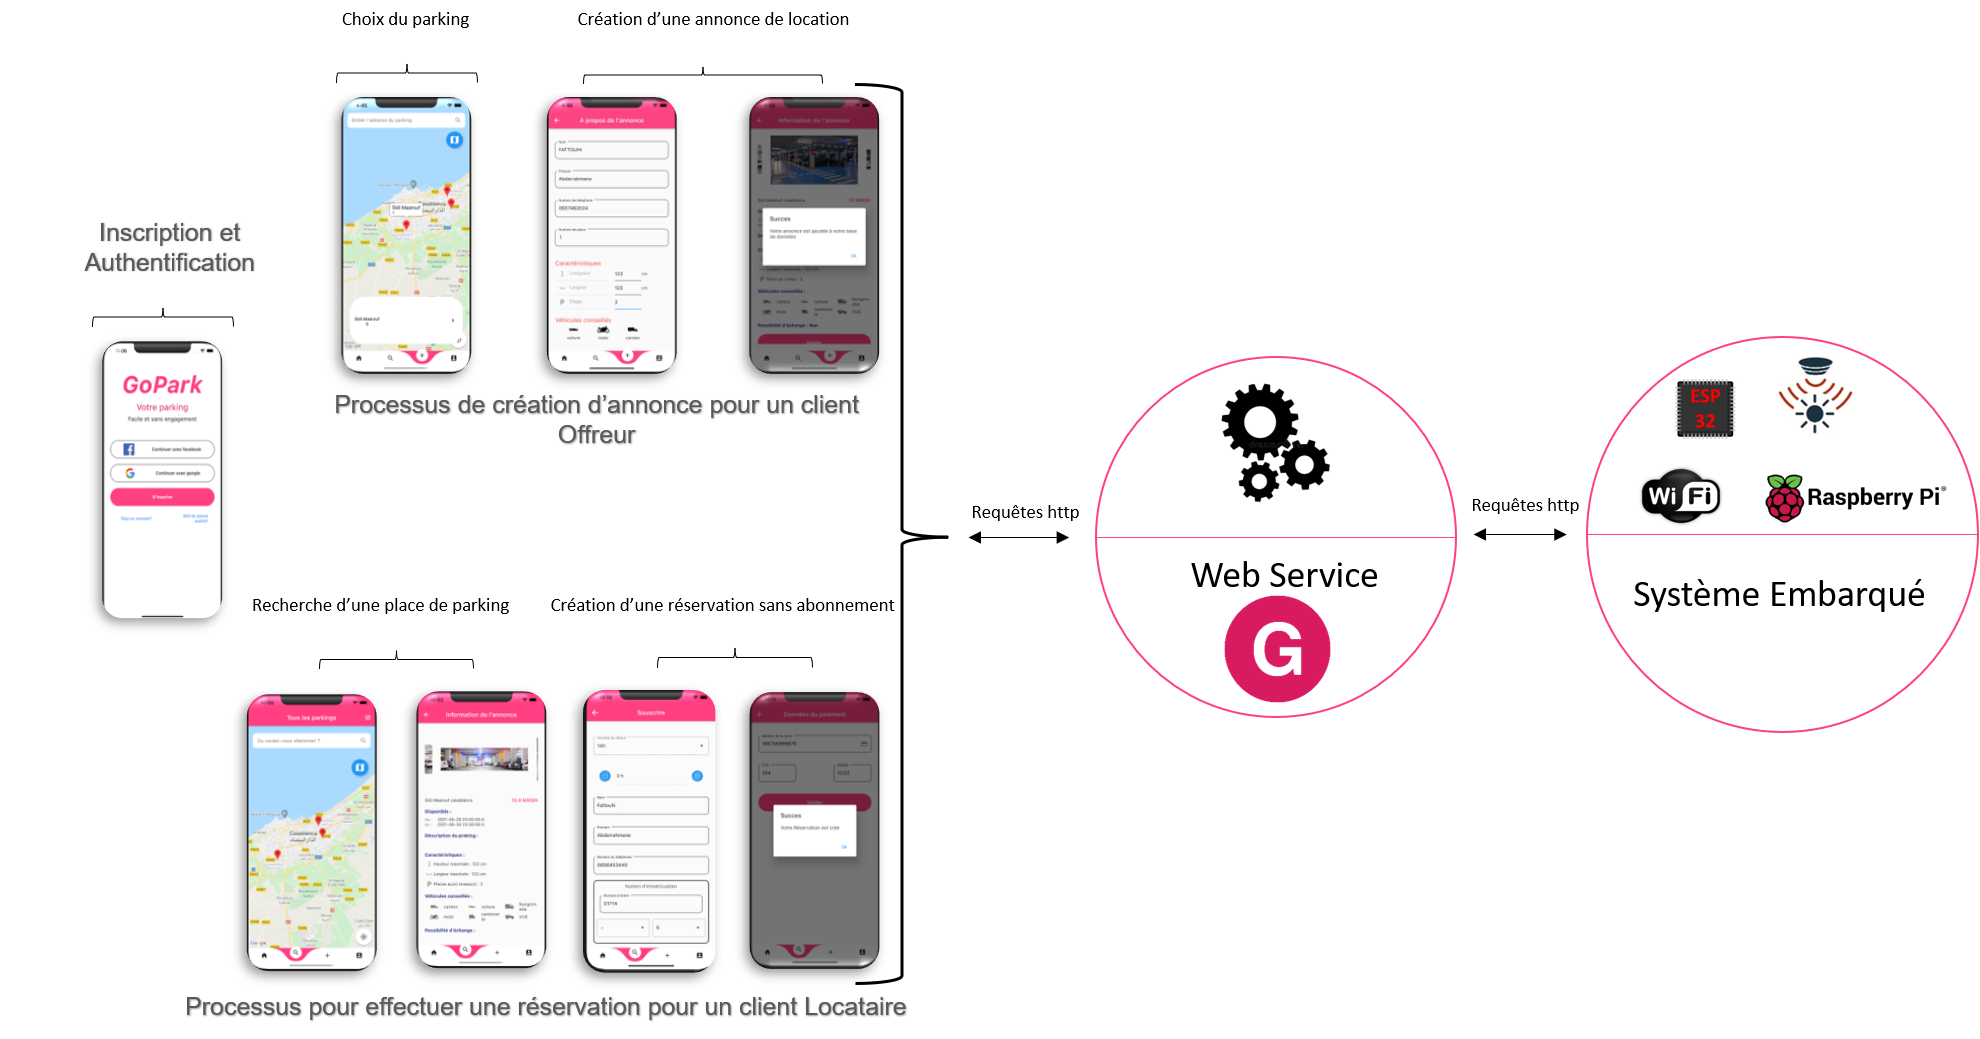
\includegraphics[scale=0.5]{goParkArchitecture.png}
        \caption{Architecture du système GoPark}
    \end{figure}

    \subsection{Environnements materiel et logiciel}
    La réalisation de la maquette de GoPark a été possible grâce à la combinaison d’un assez grand nombre d’outils matériels et logiciels. Parmi les outils matériels, on retrouve:
    \begin{enumerate}
        \item Des \textbf{capteurs ultrasoniques (1)}: ils permettent de détecter la présence d’un objet et dans notre cas la présence d’un véhicule dans l’espace de stationnement. Son principe comme son nom l’indique repose sur l’utilisation des ultrasons (ondes acoustiques). Ils sont composés d’un émetteur et d’un récepteur. L’émetteur émet régulièrement un train d’ondes qui va se réfléchir sur l’objet détecté et ensuite se rediriger vers le récepteur. Pour les deux places disponibles dans notre maquette, nous avons utilisé deux capteurs ultrasoniques.
        \item Des \textbf{microcontrôleurs (2)}: ce sont des circuits intégrés qui se composent des éléments essentiels et minimaux d’un ordinateur (processeur, mémoires, unité périphérique et interfaces entrées/sorties). Ils ont été utilisés pour le traitement avec les capteurs ultrasoniques et communiquer ainsi au serveur de l’application mobile les résultats de la détection de présence.
        \item Un \textbf{servomoteur SG90 (3)}:  c’est un actionneur qui déclenche un mouvement précis suite à une commande externe. C’est le composant qui servira à l’ouverture et la fermeture de la barrière de notre parking.
        \item Une \textbf{carte Raspberry Pi 4 (4)}: c'est un petit ordinateur (nano ordinateur) de la taille d'une carte de crédit offrant toutes les fonctionnalités d’un ordinateur standard. C’est dans cette carte que nous allons déployer notre système de reconnaissance des plaques d’immatriculation marocaines. À cette carte seront connectés le servomoteur SG90 et une \textbf{caméra V2 de 8 mégapixels (5)} pour récupérer les images de l’entrée du parking en temps réel. Voici quelques spécifications de la carte Raspberry Pi 4 que nous avons utilisée:
        \begin{table}[H]
            \centering
            \begin{tabular}{|l|l|}
                \hline
                \rowcolor{Gray}
                \textbf{Spécifications} & \textbf{Raspberry Pi 4} \\ \hline
                CPU & \textbf{1,5 GHz quadricœur ARM Cortex-A72} \\ \hline
                GPU & \textbf{Broadcom VideoCore VI, OpenGL ES 3.0} \\ \hline
                Puissance nominale  & \textbf{3A/15W} \\ \hline
                Systèmes d’exploitation & \textbf{Raspbian OS} \\ \hline
            \end{tabular}
            \caption{Spécifications de la carte Raspberry Pi 4}
        \end{table}
    \end{enumerate}
    \begin{figure}
        \centering
        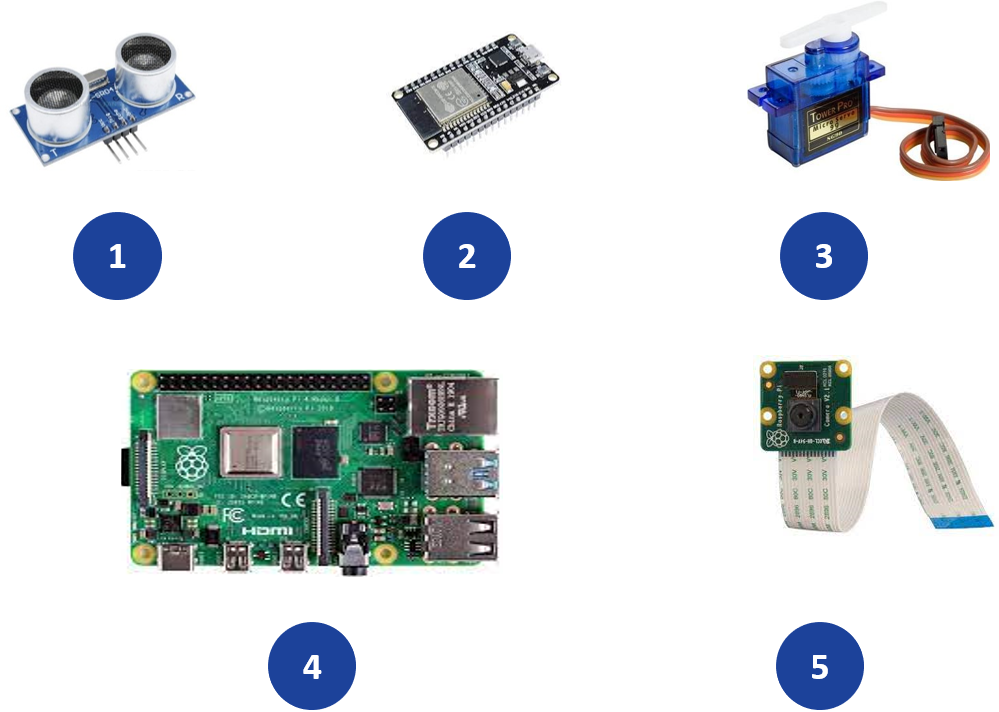
\includegraphics[scale=0.5]{materielGoPark}
        \caption{Outils matériels pour la réalisation du parking intelligent}
    \end{figure}

    Du côté logiciel, les outils dont nous nous sommes servis sont:
    \begin{enumerate}
        \item L’\textbf{IDE Arduino}: c’est une application multiplateforme qui permet d’écrire et de télécharger des programmes sur les cartes compatibles Arduino. Nous l’avons utilisé pour programmer les traitements opérés par le microcontrôleur. 
        \item Le \textbf{langage de programmation C++}: c’est le langage utilisé pour coder les programmes sous Arduino.
        \item \textbf{Firebase}: c’est un ensemble de services d’hébergement pour les divers types d'applications. Nous l’avons utilisé pour le service de base de données NoSQL qui stocke en temps réel l’état d'une place envoyée par le microcontrôleur. Par la suite, les modifications faites dans la base de données sont communiquées directement à l'application mobile.
        \item \textbf{Python}: c’est un langage de programmation interprété, multi-plateforme et multi paradigme. Au vu de sa simplicité et de la grande documentation disponible, nous avons opté pour ce langage pour coder nos programmes sur la carte Raspberry. 
        \item \textbf{OpenCV}: c’est une bibliothèque regroupant plusieurs fonctions de traitement d’images. Elle a été utile pour exécuter les différents modèles de détection et de lecture des plaques d'immatriculation sur les images en temps réel envoyées par la caméra.
        \item L’\textbf{IDE Thonny}: c'est l'éditeur utilisé pour le codage en Python.
    \end{enumerate}
    \begin{figure}
        \centering
        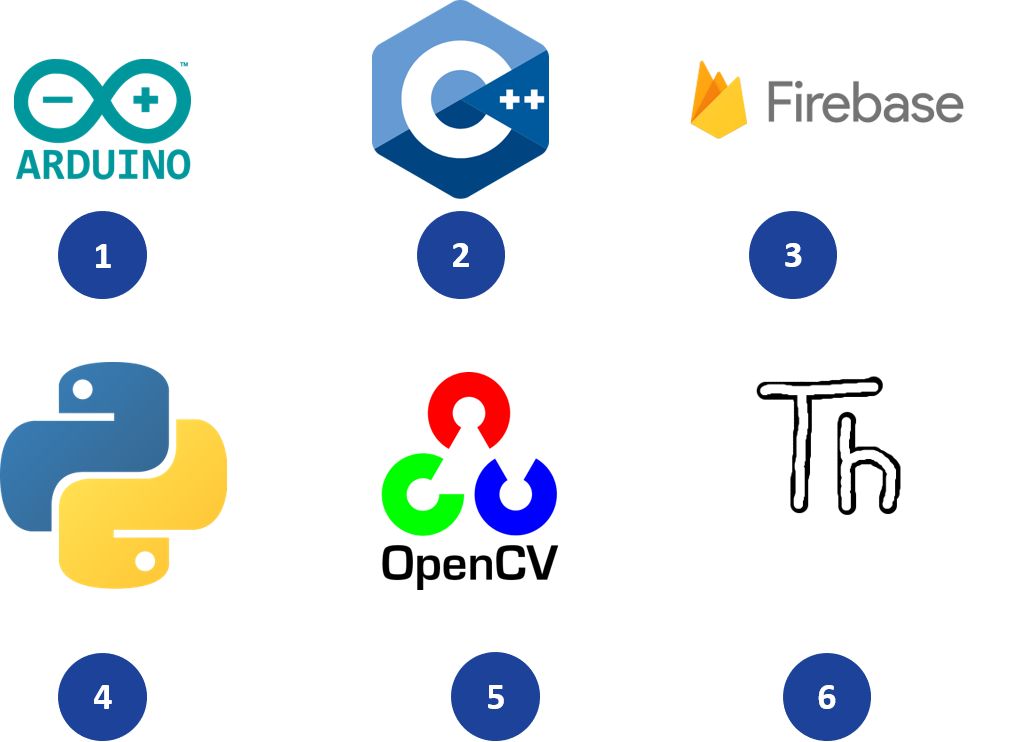
\includegraphics[scale=0.5]{logicielGoPark.png}
        \caption{Outils logiciels pour la réalisation du parking intelligent}
    \end{figure}

    \subsection{Résulats}
Le smart parking matérialisé par la maquette \ref{fig:maquette} et réalisé par notre équipe de stagiaire de KF2Y Consulting fonctionne en plusieurs étapes comme le montre la figure \ref{fig:fonctionnement}:
    \begin{enumerate}
        \item \textbf{Création d’une annonce de parking}: on accède à l’application mobile et on crée une annonce sur un parking en indiquant les places disponibles et le lieu;
        \item \textbf{Création d’une réservation}: on (en réalité un client véhiculé ) accède à l’application et fait une réservation d’une place disponible pendant une tranche horaire dans un parking présent dans les annonces sans oublier de spécifier le numéro de matricule du véhicule;
        \item \textbf{Lecture de la plaque d'immatriculation}: le véhicule se dirige à l’entrée du parking où se trouve une caméra et une barrière intelligente. La caméra envoie au programme s'exécutant sur la carte Raspberry l’image du véhicule. Le programme localise dans un premier temps la position de la plaque et par la suite extrait sous format textuel le numéro du matricule;
        \item \textbf{Vérification de l'enregistrement du matricule}: le programme s'exécutant dans la carte envoie à travers les services web REST, le numéro de matricule détecté à l’application GoPark. L’application vérifie l’existence de ce matricule dans la base de données et renvoie la réponse au programme sur la carte;
        \item \textbf{Action sur la barrière}: Si la réponse reçue par la carte est positive, on ne déclenche aucune action sur la barrière donc elle reste fermée. Dans le cas contraire, le programme déclenche immédiatement l’ouverture de la barrière pour donner accès au véhicule à la zone de stationnement;
        \item \textbf{Signalisation de l’occupation d’une place}: lorsque le véhicule arrive sur sa place de stationnement, le capteur ultrason détecte sa présence et envoie une pulsion au microcontrôleur. Ce dernier signale  cette occupation à l’application GoPark via Firebase;
        \item \textbf{Signalisation de la libération d’une place}: au moment où le véhicule libère la place, les mêmes opérations précédentes sont faites par le capteur et le microcontrôleur mais cette fois-ci pour signaler la libération d'une place.
    \end{enumerate}
    \begin{figure}
        \centering
        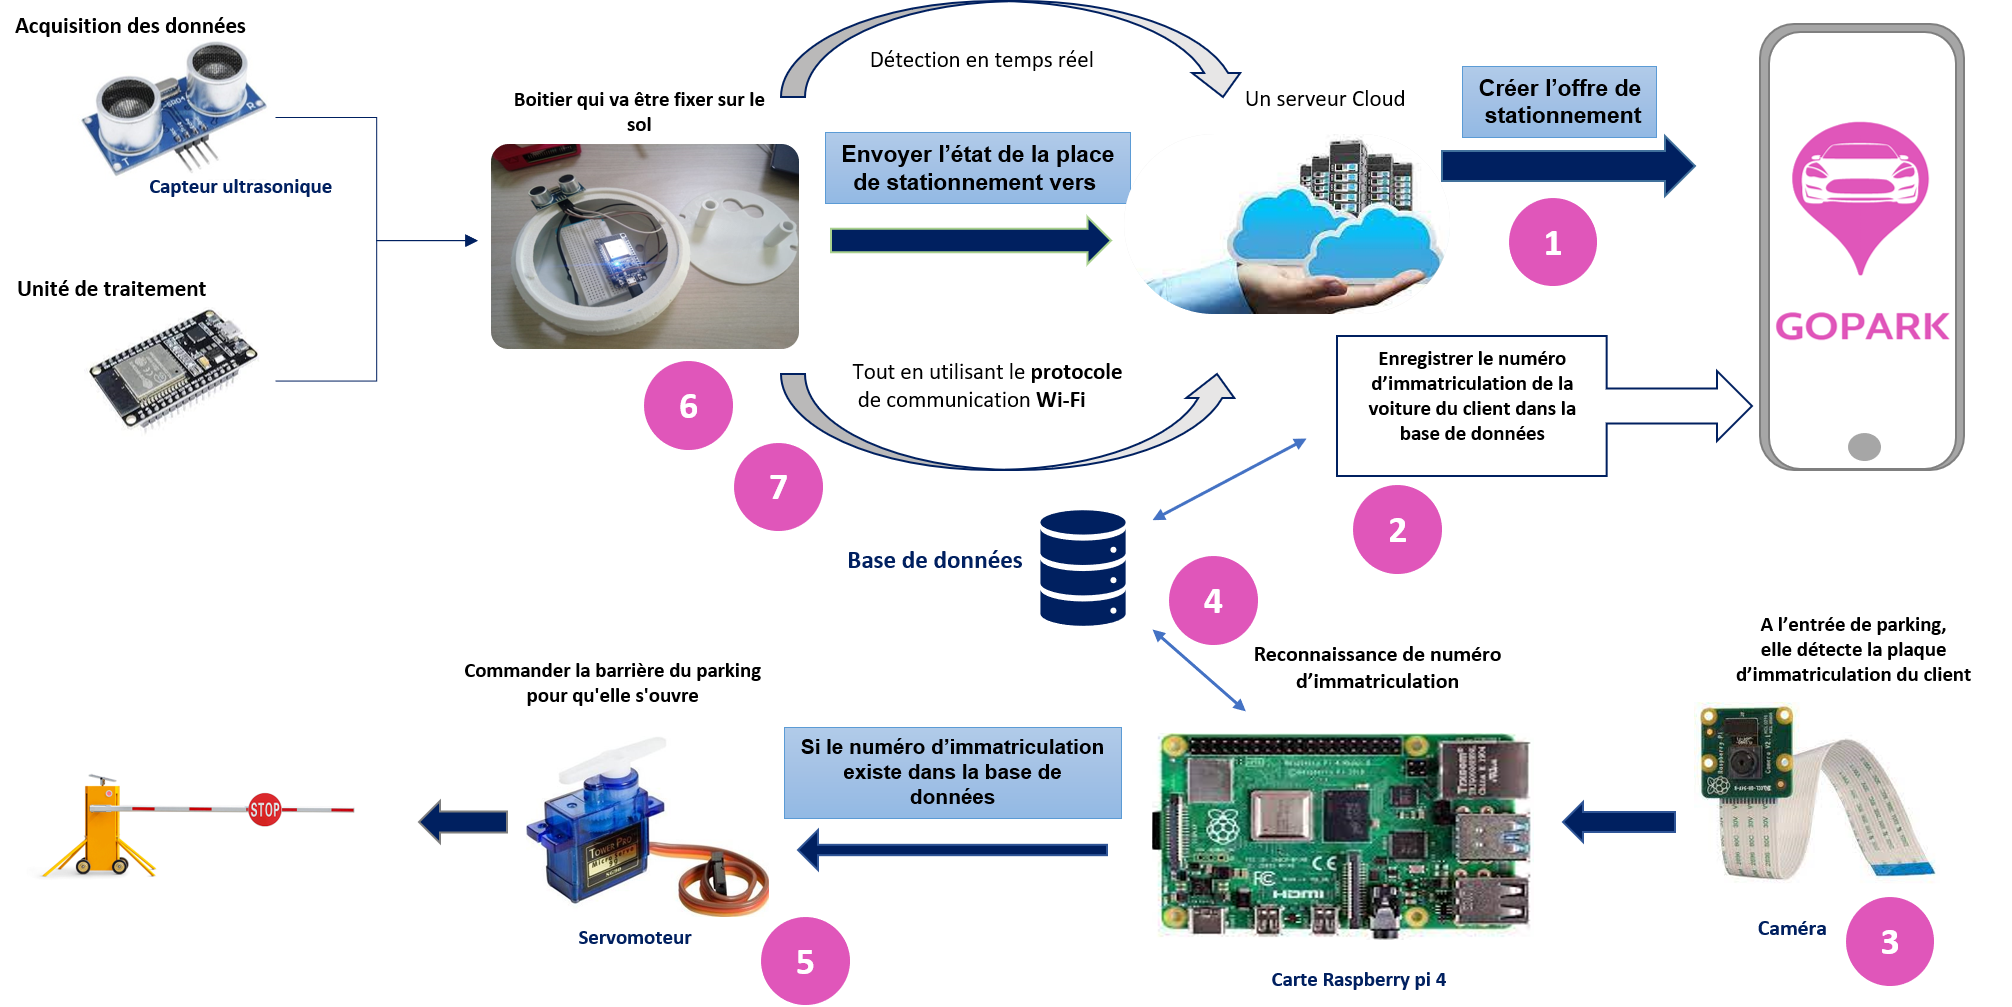
\includegraphics[scale=0.5]{goParkFonctionnement.png}
        \caption{Fonctionnement général de GoPark}
        \label{fig:fonctionnement}
    \end{figure}
    
    